
\chapter{First elements}
\section{Player selections}
The players selected several options about the campaign itself. The options
presented were based on player roles. They've chosen a Civilisation based campaign, meaning that the setting is medieval fantasy in between cities and towns. This also places them squarely on Khorvaire. The strongest motivation selected was Exploration. Some selected guilds, a nemesis, loot and a nemesis cult. 

Maaike is playing a warlock with the Infernal Pact, a forgotten devil-created path to power taught to tieflings of old. Her motivation is to find more information about this
path.

Geert-Jan will play a Thiefling himself, immediately making him a target for Maaike's curiosity. He too wants to know more of his race its origins, also so that he can fight it.

Michiel will play an Artificer. His magic, when used, looks like a holographic interface as in the Marvel Cinematic Universe. 

All three are part of the Loreseekers organisation, a group dedicated to the God of Magic, Aureon. All three have the Arcane power source. The Loreseekers find lost knowledge, often looking in faraway places such as dungeons, private collections and so forth. 

The players start in Ardev, a town in Breland. While the Loreseeker Guildmaster is in Sharn, the local branch is led by an Emeritus Loreseeker based in Ardev. Every branch has a specific region in which they attempt to recover information. A periodic update to Sharn will bring back more rewards.

We will try to play twice per week.

\begin{figure}[b]
    \centering
    \includegraphics[width=.95\textwidth]{fig/breland}
    \caption{\label{fig:breland} The map of Khorvaire around Breland.}
\end{figure}

\section{Ardev}
I've decided to make Ardev slightly bigger, with a population coming in around 3500. This is a sufficiently large population to have all possible races represented. It also makes things such as a magic shop more viable.

The city has two reasons for existing. The first is as a town close to the Royal Castle. The second is that it is a useful halfway point connecting the Droaam border to larger cities of Breland. The surrounding country is mostly flatland.

What I would imagine from such a town is that it was originally built to accomodate caravans. So, the market square should be largely central. Eventually, visiting nobility for the castle would rest or even guest here, leading to a noble district. 

The noble district is a hexagon-shaped walled district, with a circular square in the middle. The city guard is far more present in this district, and has guard posts at the three entrances. Inside, more expensive shops (read: Magical shops, armorers, etc) can be found, but they are outnumbered by the sheer amount of recreational and entertaining facilities. There is even an Opera building.

Outside, the only seemingly organised area is the main street running from the original square (Small Market) to the Noble district. This street is lined with shops. The Small Market now longer features as it did originally - one can now buy mostly fine wares there. The Large Market was made to fulfil the original, and now more numerous, purpose. It features the inns, caravansary, stables and so forth. Around both markets, the rest of the town sprawls, with many inroads. See fig~\ref{fig:ardev}.

\begin{figure}[b]
    \centering
    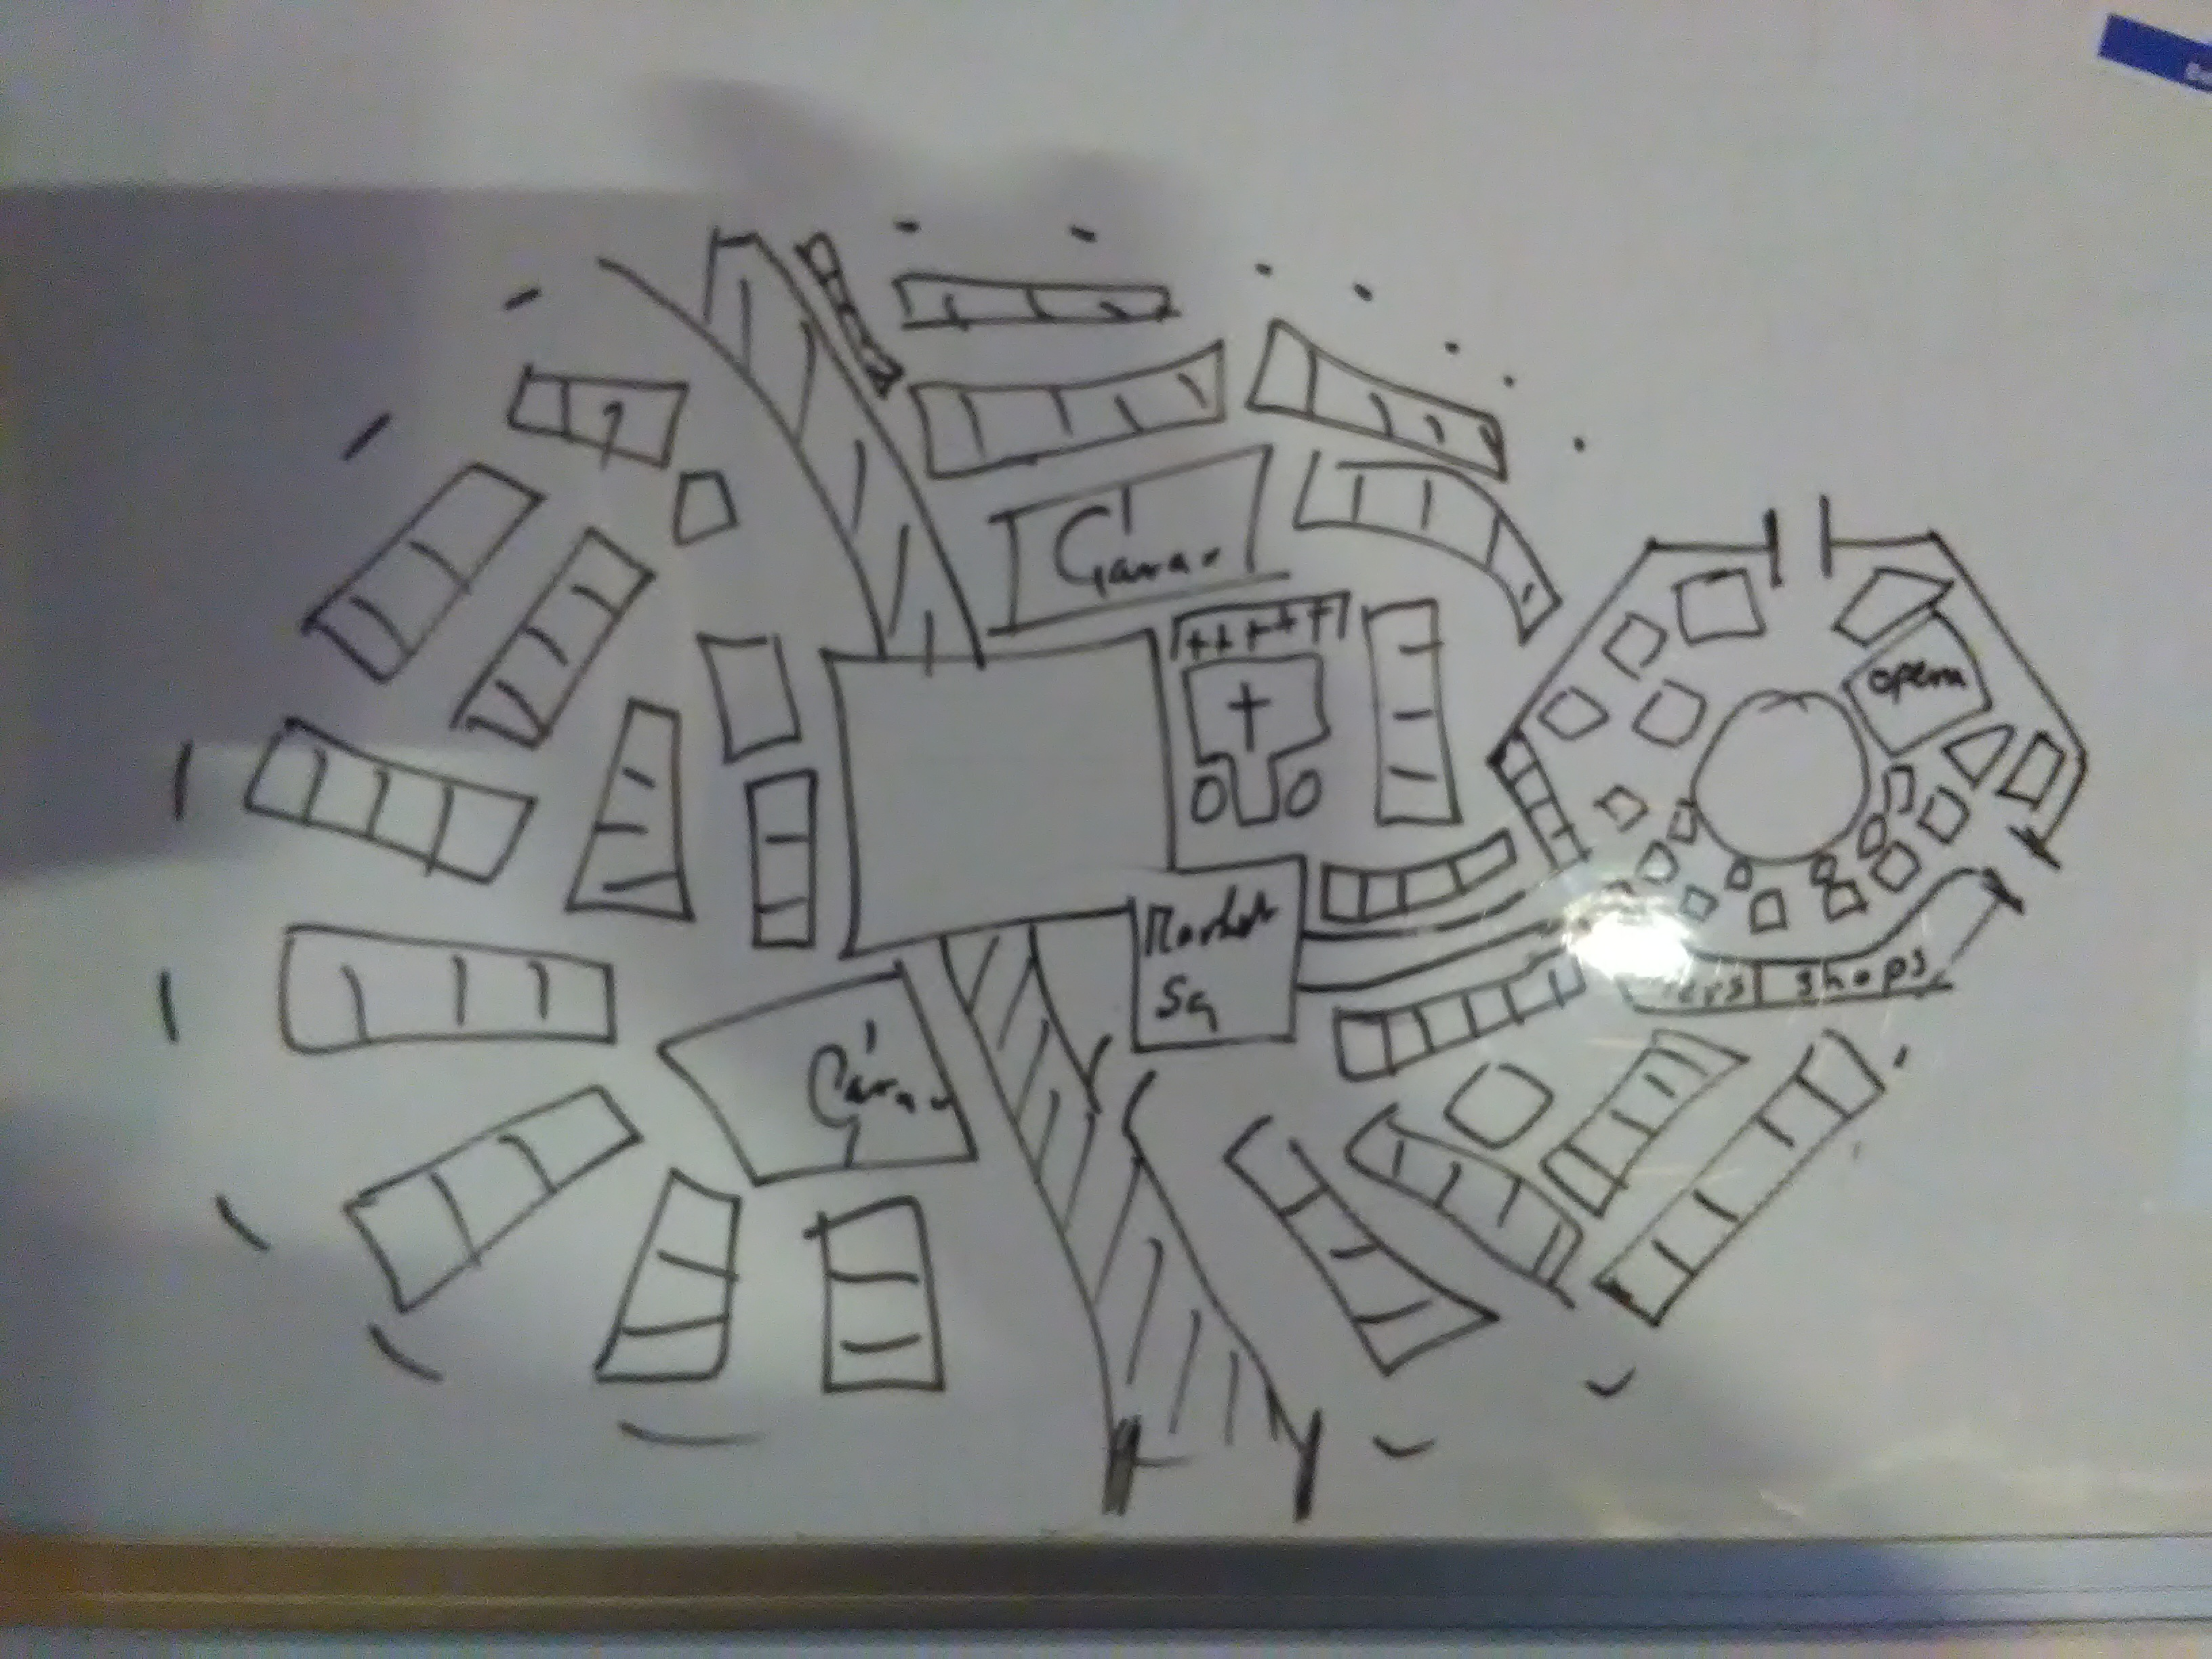
\includegraphics[width=.95\textwidth]{fig/ardev}
    \caption{\label{fig:ardev} The map of Ardev.}
\end{figure}

\section{The enemy}
The player wishes would best fit a similar group, perhaps more powerful, that is after the same interests. For this purpose, I'm putting a Thiefling Concordian (Copper Concord) crime lord at the top of the (local) nemesis group. To introduce this evil group, I need a pawn - I'm guessing that the son of the concordian would do.  The Monster vault  contains a Thiefling Brute, which would fit with the elite template applied. 

"My father told me to retrieve this book. Words aren't swords. He hit me with a book..". The Thiefling brute would be modelled after the Arishok in Dragon Age 2. A large, direct person that favours martial strength. His name is Kairon. 

My plan was to let a few of his henchmen break into the Loreseeker building. They won't find what they were looking for, but they will find the party. One enemy (a lurker) should be hit and ko'd by the Emeritus (to introduce him). This one can be questioned, to find out they were sent after a specific book. If they didn't find it, they should've reported back to a ruin, where Kairon is trying to get in to find the book his father sent for. 

The specific book is in the Emeritus' chamber. It contains information on a backentry into the ruin, allowing for a far safer entrance. Of course, when the party arrives Kairon is already inside.. As are his minions.

\section{The Emeritus}
\begin{figure}[t]
    \centering
    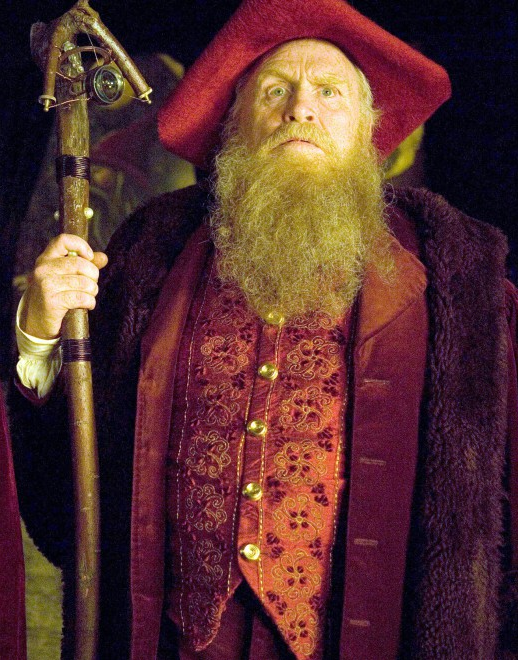
\includegraphics[width=.95\textwidth]{fig/emeritus}
    \caption{\label{fig:mustrum} The Emeritus loreseeker, Mustrum Arbelly.}
\end{figure}

The Emeritus Loreseeker is a big man. Mustrum Arbelly (fig~\ref{fig:mustrum} enjoys his retirement, spending time reading books and having lavish dinners. If the players would ever inspect the branches' finances, they'd note a rather large amount going to the Emeritus' dinners.

Mustrum also has a large number of connections - all old people know each other - and has quite some influence in the main guildhalls. However, he wanted to be near the country side, to hunt and relax. Also, he was too outspoken and brash for the majority of the main guildhall. Let's give him a ridiculously large crossbow called Bianca. Mustrum is totally not related to Archchancellor Mustrum Ridcully of the Discworld's Unseen University.

If we ignore his stature and crossbow, and his deliberate 'old people don't understand you' act, Mustrum is a powerful wizard of paragon level. Of course, nobody should know this for the very simple reason that he's retired and would like to hunt, Thank you.
